\documentclass{minimal}
\usepackage{tikz}
\usetikzlibrary{arrows,positioning} 
\tikzset{
    %Define standard arrow tip
    >=stealth',
    %Define style for boxes
    pil/.style={
           ->,
           thick,
           shorten <=2pt,
           shorten >=2pt,}
}

\begin{document}

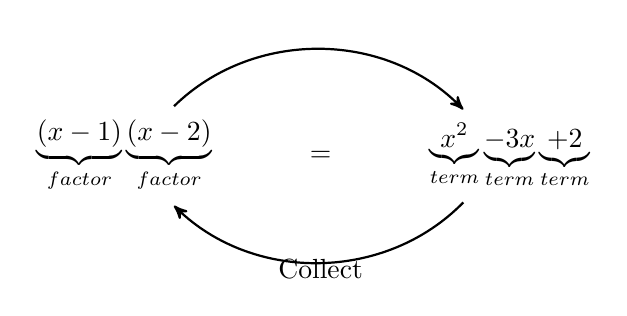
\begin{tikzpicture}[node distance=1cm, auto,]
 %nodes
 \node (collect) {Collect};
 \node[above=of collect] (eq) {$=$};
 \node [left=of eq] (factor) {$\underbrace{(x-1)}_{factor}\underbrace{(x-2)}_{factor}$};
 \node[right=of eq] (term) {$\underbrace{x^2}_{term} \underbrace{-3x}_{term} \underbrace{+2}_{term}$};

 \path (factor) edge[pil, ->, bend left=45] (term);
 \path (term) edge[pil, ->, bend left=45] (factor);

\end{tikzpicture}

\end{document}
